\documentclass{bioinfo}
\copyrightyear{2016} \pubyear{2016}

\access{Advance Access Publication Date: Day Month Year}
\appnotes{Original Paper}
\newcommand{\boldm}[1] {\mathversion{bold}#1\mathversion{normal}}

\newcommand{\ddurl}{\href{http://www.data2dynamics.org/}{http://www.data2dynamics.org/}}

\begin{document}
\firstpage{1}

\subtitle{Systems Biology}

\title[$L_1$ regularization to detect differences between cell types]{{\boldm $L_1$} regularization facilitates detection of cell type-specific parameters in dynamical systems}
\author[Steiert \textit{et~al}.]{Bernhard Steiert\,$^{\text{\sfb 1,}*}$, Jens Timmer\,$^{\text{\sfb 1,2,3}}$ and Clemens Kreutz\,$^{\text{\sfb 1,3}}$}
\address{$^{\text{\sf 1}}$Institute of Physics, University of Freiburg, Germany, \\
$^{\text{\sf 2}}$BIOSS Centre for Biological Signalling Studies, University of Freiburg, Germany, and \\
$^{\text{\sf 3}}$Freiburg Center for Systems Biology (ZBSA), University of Freiburg, Germany.}

\corresp{$^\ast$To whom correspondence should be addressed.}

\history{Received on XXXXX; revised on XXXXX; accepted on XXXXX}

\editor{Associate Editor: XXXXXXX}
% This abstract is more or less a placeholder and needs to be rewritten.
\abstract{\textbf{Motivation:}
A major goal of drug development is to selectively target certain cell types.
Cellular decisions influenced by drugs are often dependent on the dynamic processing of information.
Selective responses can be achieved by differences between the involved cell types at levels of receptor, signaling, gene regulation, or further downstream.
Therefore, a systematic approach to detect and quantify cell type-specific parameters in dynamical systems becomes necessary.\\
\textbf{Results:}
Here, we demonstrate that a combination of non-linear modeling with $L_1$ regularization is capable of detecting cell type-specific parameters.
To adapt the least-squares numerical optimization routine to $L_1$ regularization, sub-gradient strategies as well as truncation of proposed optimization steps were implemented.
Likelihood-ratio tests are used to determine the optimal penalization strength resulting in a sparse solution in terms of a minimal number of cell type-specific parameters that is in agreement with the data.
The uniqueness of the solution is investigated using the profile likelihood.
By applying our implementation to a realistic dynamical benchmark model of the \emph{DREAM6} challenge we were able to recover parameter differences with an accuracy of 78\%.
% 74\% true positives of the differences with 20\% false positives.
Within the subset of detected differences, YY\% were in agreement with their true value.
Furthermore, we found that the results could be improved using the profile likelihood.
In conclusion, the approach constitutes a general method to infer an overarching model with a minimum number of individual parameters for the particular models.
Analyzing differences between cell types enables discovering differential sensitivity to selectively target a desired cell type while leaving other cell types unaffected.
Thus, the presented methodology may alleviate directed drug design and drug development.\\
\textbf{Availability:} A MATLAB implementation is provided within the freely available, open-source modeling environment Data2Dynamics \citep{Raue2015}. Source code for all examples is provided online at \ddurl. [Please note: during the review process, the source code is available at \href{http://www.fdmold.uni-freiburg.de/~steiert/eccb/}{http://www.fdmold.uni-freiburg.de/\textasciitilde steiert/eccb/} with username `L1regularization' and password `ODEmodeling'. After acceptance, code and documentation will be incorporated into the official Data2Dynamics website \ddurl.]\\
\textbf{Contact:} \href{bernhard.steiert@fdm.uni-freiburg.de}{bernhard.steiert@fdm.uni-freiburg.de}
% \textbf{Supplementary information:} Supplementary data are available at \textit{Bioinformatics} online.
}

\maketitle

\section{Introduction}
The progress in the development of experimental assays like the establishment of high-throughput measurement techniques raised new demands on statistical methodology. 
Many scientific questions in the field of Bioinformatics and Systems Biology nowadays require large models with hundreds or even thousands of parameters or variables. 
Therefore, a major issue in many applications is feature selection, i.e. determination of informative parameters or variables, which are required to explain experimental observations, for identification of differential expression and/or for making reliable predictions. 

Selecting parameters of interest is one of the most important tasks during modeling as it heavily influences predictions.
In many cases, feature selection is equivalent to model discrimination \citep{Box67} since a set of features corresponds to a specific model with corresponding set of parameters. 
In \emph{multiple linear regression}, as an example, feature selection corresponds to choosing appropriate prediction variables used to fit an experimentally observed response variable. 
The traditional approach for choosing a suitable level of detail and the respective optimal set of features is iteratively testing many models \citep{Thompson1978}, 
i.e.~different combinations of features e.g.~by \emph{forward-} or \emph{backward selection} or combinations thereof \citep{Hocking1967, Efroymson60}. 
However, if the number of potential predictors is large, the number of possible combinations increase dramatically as shown in Figure~1\vphantom{\ref{fig:01}}, rendering such iterative procedures as infeasible. 

Regularization techniques have been suggested as an alternative approach for selecting features and fitting parameters in a single step. 
The idea is to estimate the parameters by optimization of an appropriate objective function, e.g.~by maximizing the \emph{likelihood}. 
If then, in addition, the impact of individual features is penalized, the optimal solution becomes sparse and the level of sparsity can be controlled by the strength of penalization. 
It has been shown that such penalties are equivalent to utilization of prior knowledge supplemental to the information provided by the data. 

The additional information provided by penalties reduces the variance of the estimated parameters but at the same time introduces a bias. This effect has been termed as \emph{shrinkage}. 
If the regularizing penalties are chosen appropriately, e.g. if the \emph{$L_0$}- or \emph{$L_1$-norms} are applied, a second effect occurs which can be utilized for selection. 
Because the $L_0$- and $L_1$-norm penalize parameters unequal to zero, only parameters remain in the model, which are mandatory for explaining the data. 
Since the penalized likelihood is discontinuous for $L_0$ regularization, $L_1$-penalties are usually preferred.

The concept of using the $L_1$-norm for data analysis and calibrating a model has been applied in several fields like for deconvolution of wavelets \citep{Taylor1979}, 
reconstruction of sparse spike trains of Fourier components \citep{Levy1981}, recovering acoustic impedance of seismograms \citep{Oldenburg1983} 
as well as for \emph{compressed sensing} \citep{Candes2008,Cheng2015} and clinical prediction models \citep{Hothorn2006}. 
Additionally, it has been used to establish statistical methods which are robust against violation of distributional assumptions about measurement errors \citep{Claerbout73, Barrodale1973}. Moreover, $L_1$ penalties have been applied to incorporate \emph{Laplacian priors} \citep{xx}. 
%
Despite this variety of applications, the usability for feature selection and a comprehensive statistical interpretation was not established until introduction of the 
\emph{LASSO (least absolute shrinkage and selection operator)}. 
This prominent approach for linear models was published in \cite{Tibshirani94} when the first affordable high-throughput techniques were available and the necessity of new approaches for analyzing high-throughput data became inevitable.

The standard LASSO has been generalized and adapted specifically in several directions. 
Feature selection via LASSO was discussed for the regression case in more detail in \cite{tibshirani96}, for Cox-regression in \cite{Tibshirani1997}, and for clustering e.g.~in \cite{Witten2010}.
The \emph{elastic net} has been introduced as a combination of $L_1$ and $L_2$ regularization \citep{Zou05}. 
The so-called  \emph{group-LASSO} has been established to select between predefined groups of features \citep{Yuan2006}, \emph{fused LASSO} accounts for additional constraints of pairs of parameters \citep{Tibshirani2005}, and  \emph{generalized LASSO} has been developed to regularize arbitrary prespecified parameter linear combinations \citep{Tibshirani2011}.
% Hier ist der Uebergang noch nicht smooth

Mechanistic  \emph{ordinary differential equation (ODE)} models are applied in Systems Biology for describing and understanding cellular signal transduction pathways, gene regulatory networks, and metabolism.
For such ODE models, the selection issue occurs when several cell types are considered. 
Since each cell type has different concentrations of intracellular compounds and diverse structure, each parameter of a reaction network could potentially be different. 
We suggest $L_1$-regularization in this setting to predict parameters differences between cell types.
All components of mechanistic models have counterparts in the biological pathway of interest. 
% Therefore, the models usually contain a large number of state variables representing molecular compounds and many parameters for the individual biochemical interactions. 
Therefore, the models are large and the effect of the parameters on the dynamics is typically strongly nonlinear. 
For estimating parameters in such ODE models, only a small subset of optimization routines in combination with appropriate strategies for calculating derivatives of the objective function, dealing with non-identifiability, handling of local minima etc. are applicable \citep{Raue2013}. 
We therefore augment an existing and well-tested implementation for parameter estimation for such systems \citep{Raue2015} to perform selection of cell type-specific parameters based on $L_1$-regularization. 
For this purpose, trust-region optimization \citep{Coleman96} was combined with a suitable strategy for non-linear models as presented in \citep{Schmidt09} to enable efficient optimization in the presence of $L_1$-penalties.

Since shrinkage, i.e. decreasing the variance by introducing a bias is not intended for mechanistic models, we only use $L_1$-regularization for selection, i.e. determining the cell type-specific parameters, and then use the resulting \emph{parsimonious model} to estimate the magnitude of all parameters in an unbiased manner in a second step. 
An appropriate strategy is presented for choosing the regularization strength in this setting. 
The applicability is demonstrated using a benchmark model from the \emph{DREAM (Dialogue for Reverse Engineering Assessment and Methods)} parameter estimation challenge \citep{Meyer2014}. 
The presented approach constitutes a suitable methodology for predicting cell type-specific parameters.
These could be used to predict cell type-specific sensitivities for drugs, which is a prominent challenge in cancer research.

\begin{figure}[!tpb]%figure1
\centerline{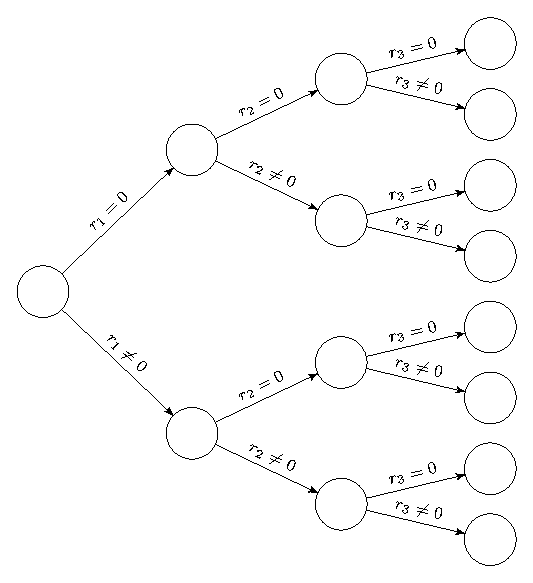
\includegraphics[width=.4\textwidth]{Figures/tree.eps}}
\caption{Na\"{\i}ve approach to select cell type-specific parameters. Each log fold-change $r_i$ of parameter $p_i$ between cell types could be either cell type-independent ($r_i=0$) or -specific ($r_i\neq 0$). Hence, the number of model candidates (circles) with grows exponentially with the number of potential cell type-specific parameters (x-axis).}\label{fig:01}
\end{figure}

\section{Problem statement}

Given a model $\mathcal M$ describing the kinetics of $c$ reaction network components $x_i$ with $i \in [1,\dots,c]$ by a system of ordinary differential equations (ODE)
\begin{equation}
\dot x(t) = f(x(t),u(t,p_u),p_x)\label{eq:ode}
\end{equation}
with a solution vector $x(t)$ representing concentrations of molecular compounds, for external inputs $u(t)$.
States $x$ are mapped to experimental data $y$ using an observation function $g$, yielding
\begin{equation}
y(t) = g(x(t),p_y)+\epsilon(\sigma(p_\sigma,x(t))) \:.\label{eq:obs}
\end{equation}
The measurement error $\epsilon \sim \mathcal N(0,\sigma^2)$ is assumed to be normally distributed in the following, although the presented approach is not limited to this assumption.
Initial concentrations $p_0$, as well as parameters $p_x$ of the ODE, $p_u$ of the input, $p_y$ of the observation function, $p_\sigma$ of the error model, are subsumed in the parameter vector
\begin{equation}
p = [p_0, p_x, p_u, p_y, p_\sigma] \:.\label{eq:par}
\end{equation}
The expressions (Eq~\ref{eq:ode}-\ref{eq:par}) fully specify $\mathcal M$.
To ensure positive values and improve numerical stability, all parameters are log-transformed.

Given data from two cell types that can be described by a common ODE structure (Eq.~\ref{eq:ode}).
The parameters $p$ are then in general specific for each cell type (ct), i.e. $p_\text{ct1} \neq p_\text{ct2}$.
However, some of the components in $p_\text{ct1}$ and $p_\text{ct2}$ may be independent from the cell type.
Discovering which of the components in $p_\text{ct1}$ and $p_\text{ct2}$ are most likely to be cell type-specific is the main topic of this manuscript.
A na\"{\i}ve approach is to simply test all possibilities for cell type-specific parameters.
However, as depicted in Figure~1\vphantom{\ref{fig:01}} the number of model candidates grows exponentially with the number of parameters, rendering such an approach as infeasible.

\subsection{Unbiased parameter estimation}

To estimate parameters $p$ for $n$ data points ${y_i}$, given the corresponding observation function observation $g(x(t_i),p_y)$ which is dependent on the ODE solution, the negative two-fold log likelihood
\begin{equation}
-2\log \mathcal L(p) = \sum_{i=1}^n \frac{(y_i-g(x(t_i),p_y))^2}{\sigma_i^2} =: \chi^2\label{eq:lik}
\end{equation}
is optimized, resulting in the maximum likelihood estimate
\begin{equation}
% \hat p = \text{arg}\min \left[ -2\log \mathcal L(p) \right] \:.
\hat p = \text{arg}\min \left[ \chi^2(p) \right] \:.
\end{equation}
In general, the ODE system cannot be solved analytically.
Therefore, numerical methods as implemented in Data2Dynamics \citep{Raue2015} are employed for calculating ODE solutions and performing maximum likelihood estimation.
Multi-start deterministic local optimization is an established approach to ensure that $\hat p$ is in fact the global optimum, as presented in \citep{Raue2013}.

\subsection{Regularization}
Regularization constitutes a prominent method to incorporate prior knowledge or to improve numerics of parameter estimation.
Here, we pursue a different strategy:
$L_k$ regularization by a penalty is used to assess the fold-change $\tilde r_i$ of parameters between cell type 1 and cell type 2, i.e. $p_{i,\text{ct2}} = \tilde r_i \cdot p_{i,\text{ct1}}$.
Therefore, the penalized likelihood
\begin{equation}
\chi^2_{L_k}(p,r) = \chi^2(p) + \lambda \sum_i ||\log \tilde r_i||_k\label{eq:likreg}%\vspace*{-4pt}
\end{equation}
is implemented consisting of the likelihood (Eq.~\ref{eq:lik}) and a $L_k$ regularization term weighted by $\lambda$.
In the following, we substitute $r_i := \log \tilde r_i$.
The regularization term corresponds to a prior in a Bayesian framework:
for $k=0$ the $L_0$ prior is a delta distribution, for $k=1$ the $L_1$ prior is a Laplacian function, and for $k=2$ the $L_2$ prior is a Gaussian function.
Using the definition
\begin{equation}
||r_i||_k := {\left( \sum_{j=1}^n |r_{ij}|^k \right)}^{1/k}\label{eq:norm}%\vspace*{-4pt}
\end{equation}
of a $L_k$-norm, we derive properties of $L_k$ for ranges of $k\in \mathbb R^+$.
$L_0$ is the apparent choice for parameter selection due to its' direct penalization of the number of $r_i \neq 0$.
However, $L_0$ is not recommended because the associated optimization problem is known to be NP-hard, i.e. the exact solution cannot be obtained within polynomial computation time.
In general, for $k<1$, the $L_k$ metric is non-convex which severely hampers numerical methods for parameter estimation.
On the positive side, $k\leq1$, for example $L_0$ and $L_1$, induce sparsity with the results usually being similar.
In contrast, the $L_k$ metric for $k>1$ does not lead to sparse results.
$L_2$, which is the metric used for the well-known least squares, can be handled efficiently but does not produce sparse results without introducing heuristics.
In that sense, the $L_1$ metric is unique because it is the only one that combines both features, convexity and sparsity.
Therefore, $L_1$ is the natural choice for parameter selection and is used in the following.
% Due to local optima, the MLE (Eq.~\ref{eq:lik}) is obtained for individual cell types.

Figure~2\vphantom{\ref{fig:02}} demonstrates how sparsity is induced by the $L_1$-norm.
In the upper row, the data contribution ($\chi^2$) is depicted by the solid black line, representing a hypothetical linear model.
The $L_1$ contribution is shown by the dashed blue lines.
With increasing $\lambda$ from panels left to right, the influence of the $L_1$ term is increased.
The lower row shows the penalized likelihood (Eq.~\ref{eq:likreg}) for $k=1$, i.e. the sum of the two lines in the corresponding upper panels.
For $\lambda=0.5$, the minimum is shifted towards zero (middle panel) in contrast to the unregularized minimum (left panel) but still different from zero.
In contrast, the minimum is exactly at zero for $\lambda=2$ (right panel).

\begin{figure}[!tpb]%figure1
\centerline{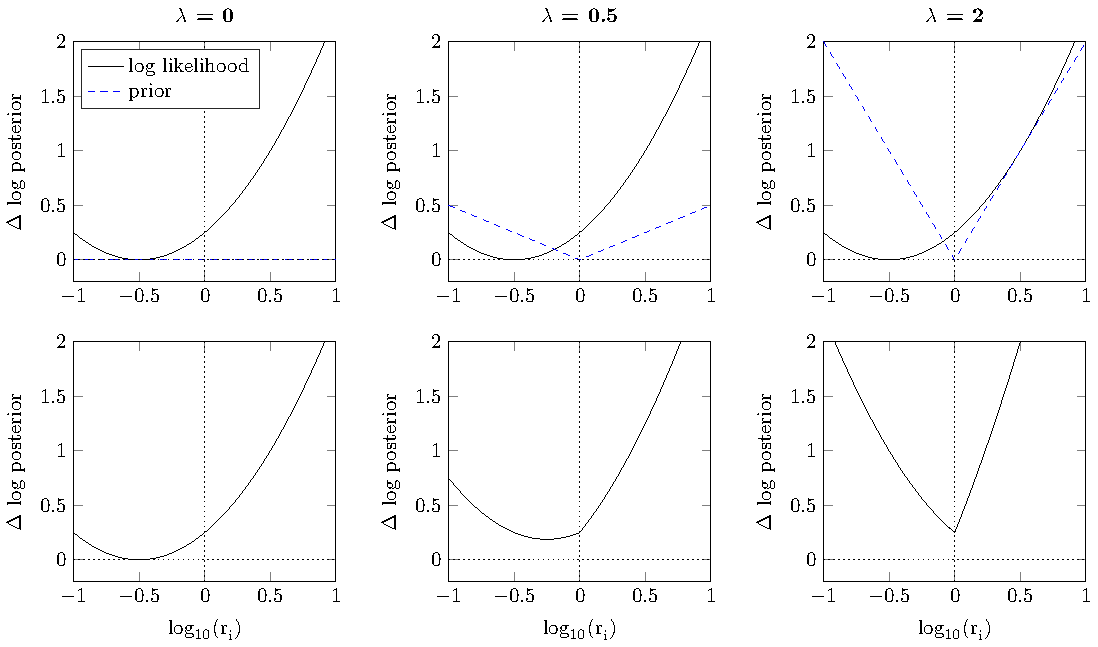
\includegraphics[width=235pt]{Figures/l1_cartoon_priorstrength.pdf}}
\caption{Sparsity and bias introduced by $L_1$ regularization. Regularization weight $\lambda$ increases from panels left to right. In the upper row, the contributions from a least-squares term ($L_2$) and an $L_1$ regularization term are shown. Their sum is plotted in the lower row. For $\lambda=0.5$, a bias is introduced shifting the minimum towards zero (middle column). When $\lambda$ is increased to 2 (left column), the minimum is exactly at zero, i.e. sparsity is induced.}\label{fig:02}
\end{figure}

\subsection{Regularized parameter estimation}
Optimization in context of partially observed stiff non-linear coupled ODEs is challenging.
However, methods have been developed to efficiently compute solutions of this problem.
To augment the existing implementations with $L_1$ regularization, i.e. to minimize the penalized likelihood
\begin{equation}
	\chi^2_{L_1}(p,r,\lambda) = \chi^2(p) + \lambda \sum_i |r_i|\label{eq:likl1}
\end{equation}
the adaptations described in the following were implemented.
Efficient optimization routines like Gauss-Newton or Levenberg-Marquardt exploit the quadratic form in (Eq.~\ref{eq:lik}).
For example, the implementation of a trust-region method \textit{lsqnonlin} in MATLAB expects residuals
\begin{equation}
	\text{res}_j = \frac{y_j-g(t_j,p)}{\sigma_j}
\end{equation}
for data points $y_j$ as input and implicitly calculates the value of the objective function by summation over squares of all residuals.
To realize optimization of the penalized likelihood (Eq.~\ref{eq:likl1}),
\begin{equation}
	\text{res}_i = \sqrt{\frac{|r_i|}{1/\lambda}}
\end{equation}
is appended to the residuals vector for each fold-change $r_i$.
The associated sensitivities
\begin{equation}
	\text{sres}_{ij} := \frac{\partial \text{res}_i}{\partial p_j} 
\end{equation}
to the regularization residuals $\text{res}_i$ are calculated as
\begin{equation}
	\text{sres}_{ii} = \frac{\text{sgn}(r_i)}{\frac{2}{\lambda}\sqrt{\frac{|r_i|}{1/\lambda}}} \:.\label{eq:sres}
\end{equation}
The gradient components
\begin{equation}
	\nabla_{r_i}\chi^2_{L_1} = 2 \: \text{res}_i \cdot \text{sres}_{ii} = \pm \lambda
\end{equation}
coincide with the slope $\pm \lambda$ induced by the $L_1$ term.
For $r_i = 0$, Eq.~\ref{eq:sres} is not defined.
In this case, the convergence criterion
\begin{align}
	&(\hat p, \hat r) = \underset{(p,r)}{\arg \max} \: \chi^2_{L_1}(p,r,\lambda) \\
	&\Leftrightarrow
	\begin{cases}
	\nabla_{p_i} \chi^2 = 0, \:\:& \text{ }\forall i\\
	\nabla_{r_i} \chi^2 + \lambda \text{ sign}(\hat r_i) = 0, \:\:& \text{ for } |\hat r_i| > 0\\
	|\nabla_{r_i} \chi^2| \le \lambda, \:\:& \text{ for } \hat r_i = 0
	\end{cases}
	\label{eq:convcrit}
\end{align}
is implemented for $r_i=0$ by setting
\begin{equation}
	\begin{cases}
	\text{sres}_{ii}=0,& \text{ for } |\nabla_i \chi^2(r_i)| > \lambda\\
	\text{sres}_{ij}=0\:\:\forall j, \:\:& \text{ for } |\nabla_i \chi^2(r_i)| \le \lambda \:.
	\end{cases}
	\label{eq:sresset}
\end{equation}
The rationale behind Eq.~\ref{eq:convcrit} is that in addition to the classical optimization criterion of vanishing gradient, the $L_1$ gradient either compensates the data gradient, or that the $L_1$ contribution dominates the data gradient and constrains the estimate to its center $\hat r_i=0$.
During optimization, this parameter-wise convergence criterion is checked for each candidate $r_i$ at every optimization step.
If the latter criterion is fulfilled, the derivative of each residual $j$ with respect to $r_i$ is set to zero, i.e. $\text{sres}_{ij}=0\:\:\forall j$.
Thereby, $r_i$ is fixed to zero for the next iteration step.
If at a certain optimization step, the convergence criterion is violated, only the $i$th $L_1$ contribution to the gradient is set to zero.
This in turn enables $r_i$ that were zero to be released during optimization if there is enough evidence in the data.
Both options are formulated in Eq.~\ref{eq:sresset}.

The $L_1$ metric has a discontinuous derivative at zero.
In other words, the optimization routine encounters sudden jumps of the derivatives as the sign of $r_i$ changes.
For $n$ parameters, there exist $2^n$ combinations of signs.
These hyper-quadrants are called orthants.
For an efficient optimization, proposed optimization steps from one orthant to another have to be avoided.
There are several methods that cope with this problem.
They have in common that they split a proposed optimization step into two:
first a step towards zero, then potentially a step away from zero.
Their major difference is the strategy how zero-values are achieved.
To mimic most of original behavior of trust-region based methods, we implemented the truncation, i.e. scaling, of an optimization step such that the orthant is maintained.
Both convergence and truncation are depicted in Figure~3\vphantom{\ref{fig:03}}.

\begin{figure}[!tpb]%figure1
\centerline{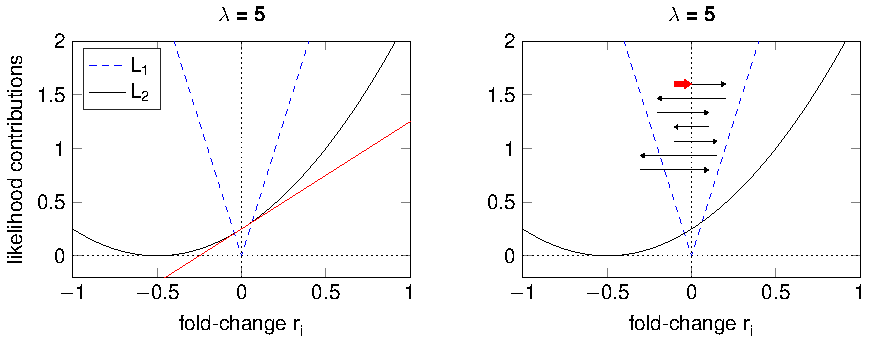
\includegraphics[width=235pt]{Figures/l1_cartoon.pdf}}
\caption{Convergence criterion and truncation for an optimum of $\chi^2_{L_1}$ at zero. Left panel: the implementation considers a $L_1$ regularized parameter $r_i=0$ to be converged if the gradient from the data ($\chi^2$ - black line) is smaller than the slope of the $L_1$ term (dashed blue line). For $r_i=0$, the algorithm compares the red line, which is the slope of the black line at this point, to the blue dashed line. In this example, the slope of the $L_1$ term is larger than of the $\chi^2$ term, hence the minimum is at zero and the corresponding entries in the sensitivity matrix are set to zero. Right panel: The black arrows from top to bottom give a cartoonish representation of optimization steps. To avoid jumping back and forth (black arrows), i.e. numerical instability by changing the sign of $r_i$ due to discontinuously changing slope of $L_1$, optimization steps are truncated to the boundary of the orthant as indicated by the red arrow.}\label{fig:03}
\end{figure}

\subsection{Regularization strength $\lambda$}
To choose the optimal value $\lambda^*$ of the regularization strength, $\lambda$ is increased from 0 and the un-regularized likelihood is re-optimized until mismatch between model and data is too large to not reject the associated simplification.
% This strategy is similar to the calculation of \emph{PL}, where a parameter of interest is fixed and the remaining parameters are re-estimated.
Thus, likelihood-ratio statistics are employed to discover admissible values.
For $L_1$ based parameter selection, cross validation has been suggested to choose the final value for the regularization weight $\lambda$.
However, for nonlinear models, leaving data out could produce non-identifiablilites and the effect on the prediction error can be ambiguous.
Therefore, we decided to use an information theory based test criterion.
The most prominent methods are the likelihood ratio test (LRT), the Akaike information criterion (AIC), and the Bayesian information criterion (BIC).
% The criteria are depicted by the vertical lines in Figure~4\vphantom{\ref{fig:04}} for an exemplary regularization path.
In certain settings these are equivalent:
AIC resembles LRT for fixed $\alpha = 15.6\%$ and $1$ degree of freedom.
Further, AIC is known to select systematically too large models and is thus not a consistent model selection criterion.
% With growing model size, $\alpha$ should be adjusted.
% As this is not the case for AIC, we favor LRT over AIC.
BIC considers the number of data points and is a consistent model seletion criterion.
Moreover, BIC is equivalent to LRT with adjusted $\alpha$ level.
Therefore, we only use LRT in the following without loss of generality.

For certain values of $\lambda$, each $r_i$ is estimated either to zero or non-zero by optimizing Eq.~\ref{eq:likl1}.
% In a second step the $L_1$ regularization is omitted and 
Then, using Eq.~\ref{eq:lik} the unbiased maximum likelihood estimate is calculated, under the side constraint that fold-changes with $r_i=0$ are fixed to zero.
The value of the objective function for this constrained unbiased solution is denoted as $\chi^2_\lambda$.
The LRT statistics
\begin{equation}
	D(\lambda) = \chi^2_\lambda - \chi^2_{\lambda=0}
\end{equation}
quantifies the discrepancy to the full model with solely cell type-specific parameters.
The cut-off for determining the \emph{parsimonious model}, i.e. the model with a minimal number of differences for a given $\alpha$ level which allows fitting the data is given by the $\chi^2_{m_\lambda,\alpha}$ distribution with degrees of freedom $m_\lambda=\#r_i - \#(r_i=0)_\lambda$.
Thus the \emph{parsimonious model} is given by
\begin{equation}
	\lambda^* = \arg \lceil D(\lambda) < \chi^2_{m_\lambda,\alpha} \rceil \:.
\end{equation}
We use the significance level $\alpha = 0.05$ in the following.
% At the end, a good method should optimize specificity and sensitivity.
% Thus, the result should appear as far as possible to the upper-left corner of the ROC curve.

\subsection{Profile likelihood}
The \emph{profile likelihood (PL)} constitutes a method to calculate confidence intervals (CI) of parameters or predictions, see \cite{Raue2009} and \cite{Kreutz2012} for an overview.
It only requires weak assumptions and therefore performs well even for strongly non-linear problems where asymptotic methods based on the Fisher Information matrix fail.
The basic idea is to fix a certain model quantity of interest, e.g. a parameter, and re-optimize all remaining parameters. % Formula?
This re-optimization procedure is iterated for different fixed values of the quantity of interest.
By comparing the increase in $\chi^2$ with respect to the maximum likelihood the CI is calculated.

Here, we use the \emph{PL} to check the parameter differences discovered by our $L_1$ based implementation.
Thus, the un-regularized \emph{PL} of a fold-change parameter $r_i$ that has been proposed using $L_1$ regularization is calculated.
If selection was successful, the \emph{PL} should not be compatible with 0.
This interpretation is equivalent to a likelihood ratio test between the null model $r_i=0$ and the alternative model $r_i \neq 0$.
% However, the results are not expected to match exactly due to parameter dependencies that prevent $r_i=0$ for the regularized problem.
Note that we did not use \emph{PL} in the first place, as the combinatorial issue shown in Figure~1\vphantom{\ref{fig:01}} is not solved by this approach.

In addition, the \emph{PL} can be used to investigate the uniqueness of the solution.
In a non-unique setting there are multiple alternatives to select parameter differences.
For instance, a selected cell type-specific parameter could be exchanged with another parameter that was not selected as different.
For testing uniqueness, the \emph{PL} for each $r_i$ with estimate $\hat r_i=0$ is calculated.
This is equivalent to testing a model with one additional parameter ($r_i$) in comparison to the \emph{parsimonious model} ($r_i \equiv 0$).
If inside the CI of $r_i$, another parameter that was different to zero is now compatible with zero, one cannot decide based on the given data which one is different.

%Finally, regularized \emph{PL} of selected differences can pinpoint compensating effects.
%Compensation manifests in piecewise flat regions in \emph{PL} though the regularization alone should already induce non-zero derivatives of \emph{PL}.
%However, if a parameter change is compensated by adjusting another parameter, the regularizations can cancel out as well.
%The \emph{PL} shape is then a clear indicator for compensation.

\begin{methods}
\section{Approach}
The approach presented in this manuscript extends the available methodology implemented in the modeling environment Data2Dynamics \citep{Raue2015} by $L_1$ regularization.
Data2Dynamics has been used in a variety of applications \citep{Becker1404,Bachmann516,Beer2014} to perform parameter estimation, uncertainty analysis, and experimental design of nonlinear stiff partially observed ODE systems.
In the following, we summarize the $L_1$ specific enhancements in addition to the established modeling routine as implemented in our approach for discovering cell type-specific parameters.

Given an overarching model that is able to describe two cell types with two independent parameter vectors $p_\text{ct1}$ and $p_\text{ct2}$ for cell types 1 and 2, respectively.
Fold-changes $r_i$ are calculated to express the parameters of cell type 2 relative to cell type 1, i.e. $p_{i,\text{ct2}} = \tilde r_i \cdot p_{i,\text{ct1}}$.
Eq.~\ref{eq:likl1} is used to $L_1$ penalize deviations of the fold-change parameter vector $r$ to zero.
In contrast to many other \emph{LASSO}-like techniques, our method consists of two consecutive steps:
\begin{enumerate}
\item Using the regularized $\chi^2_{L_1}$ to determine cell type-specific parameters 
\item Using the un-regularized $\chi^2$ to determine the \emph{parsimonious} model and parameter estimates 
\end{enumerate}
For the first step, $\lambda$ is scanned and the cell type-specific parameters are determined for each value of $\lambda$.
Then, at the second step, for choosing the optimal $\lambda^*$ the un-regularized Eq.~\ref{eq:lik} is optimized, under the constraint that parameters with $r_i = 0$ are shared between both cell types.
The full model with all parameters specific for each cell type is compared by the likelihood ratio test to each of the models that were selected using $L_1$ regularization.
Thereby, the \emph{parsimonious model} is defined as the minimal unbiased model that cannot be rejected by the likelihood ratio test.

To cope with diverging terms in the Hessian matrix, we implemented a heuristic that tests each $L_1$ parameter against zero in order by their magnitude of deviation from zero.
If the likelihood did not increase by more than one, the correction was accepted.
Potential improvements to such a strategy are provided in the discussion.

Alternatively, the \emph{PL} can be utilized to further reduce the number of cell type-specific parameters, which we illustrate exemplarily.
In addition, we show investigation of uniqueness using the \emph{PL}.
However, it is not feasible to perform these calculations for each of the $N=500$ runs, because obtaining such a large number of \emph{PL} is computationally not feasible for the given model size.
When applied in practice, results can be further improved by the presented analyses pointing out even smaller and biologically more plausible solutions.

% Further, plotting unobserved components for both cell types enables validation design by discovering dynamics with a small prediction CI, which are different between the cell types.

%Text Text Text Text Text Text  Text Text Text Text Text Text Text
%Text Text Text Text Text Text Text Text.
%Figure~2\vphantom{\ref{fig:02}} shows that the above method  Text
%Text Text Text Text Text Text Text Text Text  Text Text.
%\citealp{Boffelli03} might want to know about text text text
%text\vspace*{1pt}
%
%\begin{itemize}
%\item for bulleted list, use itemize
%\item for bulleted list, use itemize
%\item for bulleted list, use itemize\vspace*{1pt}
%\end{itemize}
%
%Text Text Text Text Text Text  Text Text Text Text Text Text Text
%Text Text Text Text Text Text Text Text.
%Figure~2\vphantom{\ref{fig:02}} shows that the above method Text
%Text Text Text Text Text Text Text Text Text Text Text.
%\citealp{Boffelli03} might want to know about text text text text
%Text Text Text Text Text Text  Text Text Text Text Text Text Text
%Text Text Text Text Text Text Text Text.
%
%Text Text Text Text Text Text  Text Text Text Text Text Text Text
%Text Text  Text Text Text Text Text Text\vadjust{\newpage}.
%Figure~2\vphantom{\ref{fig:02}} shows that the above method  Text
%Text Text Text  Text Text Text Text Text Text  Text Text.
%\citealp{Boffelli03} might want to know about text text text text
%
%
%\subsection{This is subheading}
%
%Text Text Text Text Text Text Text Text Text Text Text Text Text
%Text Text  Text Text Text Text Text Text.
%Figure~2\vphantom{\ref{fig:02}} shows that the above method  Text
%Text Text Text Text Text Text Text Text Text  Text Text.
%\citealp{Boffelli03} might want to know about  text text text text
%Text Text Text Text Text Text  Text Text Text Text Text Text Text
%Text Text  Text Text Text Text Text Text.
%
%
%\subsubsection{This is subsubheading}
%
%Text Text Text  Text Text Text Text Text Text  Text Text.
%\citealp{Boffelli03} might want to know about  text text text text
%Text Text Text Text Text Text Text Text Text Text Text Text Text
%Text Text  Text Text Text Text Text Text.
%Figure~2\vphantom{\ref{fig:02}} shows that the above method  Text
%Text Text Text  Text Text Text Text Text Text  Text Text.
%\citealp{Boffelli03} might want to know about  text text text text
%
%\enlargethispage{6pt}
%
%
%Text Text Text Text Text Text  Text Text Text Text Text Text Text
%Text Text  Text Text Text Text Text Text.
%Figure~2\vphantom{\ref{fig:02}} shows that the above method  Text
%Text Text Text  Text Text Text Text Text Text  Text Text.
%\citealp{Boffelli03} might want to know about  text text text text


\end{methods}

%\begin{figure}[!tpb]%figure2
%%\centerline{\includegraphics{fig02.eps}}
%\caption{Caption, caption.}\label{fig:02}
%\end{figure}

%Text Text Text Text Text Text  Text Text Text Text Text Text Text
%Text Text  Text Text Text Text Text Text.
%Figure~2\vphantom{\ref{fig:02}} shows that the above method  Text
%Text Text Text  Text Text Text Text Text Text  Text Text.
%\citealp{Boffelli03} might want to know about  text text text text\vspace{10pt}

\section{Application}
\subsection{Model description}
In the following, we use model \emph{M1} from the \emph{DREAM6 (Dialogue for Reverse Engineering Assessment and Methods)} challenge as benchmark for our approach \citep{Steiert12}.
The model represents a gene-regulatory network and was chosen because it enables testing many observation setups and parameter differences.
It was used in 2011 to evaluate the performance of experimental design strategies to optimize parameters and predictions.
The model incorporates transcription and translation of six genes.
Therefore, the dynamic variables represent six mRNAs, as well as the six associated proteins with known initial concentrations.
Genes can positively and/or negatively regulate each other.
Taken together, the model consists of 29 parameters.
13 are associated with synthesis and degradation of molecules:
1 protein degradation rate which is shared among all proteins; 
6 ribosomal strengths determining the synthesis rate of mRNAs;
6 protein synthesis strengths which define how strong mRNA presence induces protein production;
The remaining 16 parameters define the interaction of genes by Hill kinetics, thus 8 $K_D$ values and 8 Hill coefficients are assumed.

\emph{DREAM6 M1} was simulated with gold-standard parameters that were made publicly available after completion of the challenge.
We now use this gold-standard as cell type 1.
When complete data is provided, i.e. all observables measured at all possible experimental conditions, all parameters are identifiable, except for one Hill coefficient which is only restricted to lower values.
Thus, we conclude that determining parameter differences between cell types is possible in principle.
Next, we assumed 1/3 of all parameters to be cell type-specific.
We therefore randomly simulated fold-changes of $[1/10~1/5~1/2~2~5~10]$ for non-Hill parameters.
For Hill coefficients, fold changes of $[1/4~1/2~2~4]$ were assumed such that Hill coefficients are within the interval $[1,4]$ for both cell types.
This range is motivated biologically as thereby the number of binding sites on a molecule is considered.
Taken together, the number of possible models is $2^{29}$, i.e. more than $10^8$.

We chose the following two observation types from the original \emph{DREAM6} challenge setup:
(1) mRNA measurements for all mRNAs with 21 data-points each, and (2) protein measurements for 2 selected proteins, each with 41 data-points.
The observation function is the identity, i.e. the molecular compounds are observed directly without scaling or offset parameters.
The error model contains an absolute term as well as a relative term with fixed weighting.
% If a trajectory was near zero, negative data points may occur which were then set to zero to avoid negative concentrations.
In addition to wildtype data, there is the option of performing 3 possible perturbations for each of the six nodes:
\begin{enumerate}
\item knock-out ($\text{mRNA\_pro}_i=\text{Prot\_pro}_i=0$)
\item knock-down ($\text{mRNA\_deg}_i\rightarrow 5\cdot \text{mRNA\_deg}_i$)
\item over-expression ($\text{mRNA\_pro}_i \rightarrow 2\cdot \text{mRNA\_pro}_i$)
\end{enumerate}
In total, this results in 18 possible experimental conditions.
To have a reference for perturbations wildtype data, i.e. mRNA and protein data for all observables, was included for parameter estimation.
Within the challenge, an identifiable setting has been achieved using 9 additional data sets out of 331 possibilities.
To allow variability in the number of experiments, we randomly (50\%) selected for each of the 18 conditions whether it was observed or not.
To mimic the partial observation which was one task of the \emph{DREAM6} challenge, we chose randomly whether mRNA (1/3) or proteins (2/3) were observed.
Given the latter, 2 out of 6 proteins were randomly selected.
We chose the same experimental conditions and observables for both cell types.

After implementing the fold-changes between cell types, as well as perturbations and observations we used a $L_1$ regularization for all fold-change parameters and scanned along $\lambda$ for parameter selection.
To chose the optimal regularization strength $\lambda^*$ we used the un-regularized $\chi^2$.
Thus, we could select the \emph{parsimonious model} and ensure unbiased estimates of the fold-change parameters.

\begin{figure}[!tpb]%figure1
\centerline{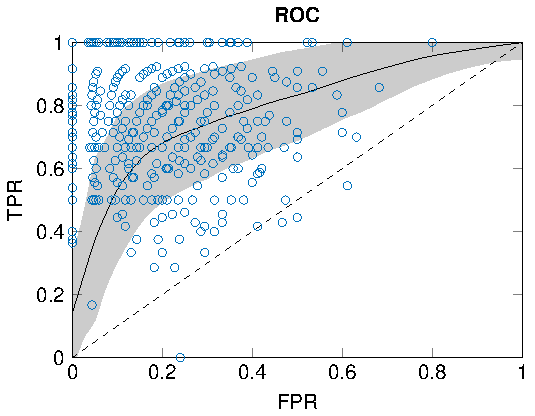
\includegraphics[width=235pt]{Figures/ROC.pdf}}
\caption{Averaged ROC curve. For each of the $N = 500$ runs, the ROC curve is calculated in dependence of $\lambda$. The black line depicts the arithmetic mean ROC curve and the shading the standard deviation. Blue circles denote the selected model for each repetition. Because the dots appear on average near the maximum of sensitivity and specificity (upper left corner), we consider the selection criterion as appropriate.}\label{fig:04}
\end{figure}

\subsection{Performance assessment}
The procedure of selecting fold-changes and observations was repeated $N=500$ times. % , yielding a random sample of $2^{29} \cdot 331 > 10^{11}$ possibilities.
Afterwards, the presented algorithm for $L_1$ regularized parameter selection was applied in an unsupervised manner.
The performance is summarized in Figure~4\vphantom{\ref{fig:04}}.
For each run, a receptor operating characteristic (ROC) curve is calculated by scanning $\lambda$ from $10^{-4}$ to $10^6$.
The black line depicts the arithmetic mean ROC curve and the shading the standard deviation over all $N=500$ repetitions.
The blue dots show the \emph{parsimonious model} selected by the likelihood-ratio test.
Usually, for a given ROC curve the selection criterion is chosen to maximize both sensitivity and specificity simultaneously, which is the point most up-left on the ROC curve.
Because the blue dots appear centered around this `kink', we consider the selection criterion appropriate.
On average, the implementation results in a 74\% true positive rate (TPR) and a 20\% false positive rate (FPR) for the given setting.
The overall accuracy is 78\%.
Despite this imperfect accuracy and related classification errors, XX\% out of the true positives were estimated closest to their true fold-change.
Thus, we conclude that the strategy to calculate unbiased estimates for selected fold-changes is robust against missclassification.

We further evaluated the performance of our $L_1$ fold-change detection routine for different parameter types.
The results are summarized in Table~1\vphantom{\ref{Tab:01}}.
The protein degradation rate is shared among all proteins.
It is detected in 100\% as different when there was a difference simulated.
On the other hand, this parameter also had the highest FPR with approximately 46\%.
A possible explanation is given by the fact that our method is data driven and hence differences are more likely to be detected in points of the network with more data available.
This is the case for the protein degradation rate because it influences all proteins in the network.
The individual protein production and ribosomal strengths have a FPR around 20\% and a TPR of approximately 80\%.
In contrast, the Hill regulation parameters ($K_D$ and Hill coefficient) are detected less frequently as different.
Probably, this is due to identifiability issues as those parameters were already the most difficult ones to estimate in the original \emph{DREAM0}6 challenge.
The underlying reason is that the concentration range around $K_D$ has to be sampled for a reliable estimation, which cannot be ensured without proper experimental design.

% Performance for different fold-changes\\ % Wie bewertet man das am besten? Braeuchte man evtl. Unsicherheitsabschaetzungen ...
% Performance for different ratio of protein vs mRNA measurement % Ist das spannend?

\begin{table}[!t]
\processtable{Performance of algorithm for \emph{DREAM6 M1}\label{Tab:01}} {\begin{tabular}{@{}llllll@{}}\toprule Parameter class &
$N_\text{test}$ & $N_\text{mod}$ & FPR & TPR & ACC\\\midrule
Protein degradation rate & 500 & 181 & 0.4577 & 1.0000 & 0.7080\\
Protein production strength & 3000 & 1032 & 0.2393 & 0.7965 & 0.7730\\
Ribosomal strength & 3000 & 986 & 0.1927 & 0.7982 & 0.8043\\
$K_D$ value & 4000 & 1365 & 0.1624 & 0.6989 & 0.7903\\
Hill coefficient & 4000 & 1311 & 0.1852 & 0.6461 & 0.7595\\\hline
All & 14500 & 4875 & 0.2006 & 0.7366 & 0.7783\\\botrule
\end{tabular}}{On average, 1/3 of the parameters that could potentially be cell type-specific ($N_\text{test}$) were drawn to actually be cell type-specific ($N_\text{mod}$). Overall, parameter differences are detected with 78\% accuracy. The model containts a shared degradation rate for all proteins, which is often diagnosed as different. Protein production and ribosomal strengths are on average for FPR and TPR. $K_D$ and Hill coefficients are difficult to detect because concentration range around $K_D$ has to be covered to see effect on dynamics. 500 repetitions were computed. Each run ($L_1$ regularized scan and subsequent unregularized scan to identify \emph{parsimonious model}) took 28.8 min on average on an Intel Xeon E5-1620 3.60Ghz desktop computer.}
\end{table}

\subsection{Supervised examination} % Hier noch klarer machen, was genau gemacht werden soll.
In the following, we select one representative setup out of the $N=500$ given by a minimal deviation of its ROC curve to the average ROC curve.
% For the automatic model selection shown in the previous section, $\lambda$ was scanned around the selected value.
% Now, we use a higher resolution for $\lambda$.
The regularization path is plotted in the left panel of Figure~5\vphantom{\ref{fig:05}}.
With increasing $\lambda$, fold-change parameters are shrinked towards zero, and at some point eventually estimated exactly to zero.
Thus, the number of cell type-specific parameters decreases for larger $\lambda$.
The dependency of the likelihood ratio, i.e. the decrease of the unregularized $\chi_\lambda^2$ compared to the full model with only cell type-specific parameters, is shown by the blue line in the right panel of Figure~5\vphantom{\ref{fig:05}}.
The statistical threshold $\chi^2_{m_\lambda,0.05}$ is depicted by the dashed red line.
The regularization strength $\lambda^*$ at which both lines cross marks the \emph{parsimonious model} that has minimal complexity but cannot be statistically rejected.

% Next, we calculate \emph{PL} for each regularized parameter to check for compensating effects.
We checked by calculating \emph{PL} of the unregularized fold-change parameters whether the results are not compatible with zero (Figure~6\vphantom{\ref{fig:06}}).
False positive fold changes (parameters 1, 4, and 5) are depicted by the red boxes.
When the \emph{PL} (black line) crosses zero (black vertical dashed line) below the statistical threshold (red horizontal dashed line), the parameter is a candidate for supervised removal.
Here, this enables the detection of three additional parameters which could be independent from cell type.
Interestingly, all these were false positives.
In comparison to the automatically detected parameter differences, the result of the supervised examination decreased the FPR from XX\% to YY\% and increased the TPR from XX\% to YY\%.
We elaborate more detailed on the consequences of this result in the discussion.

Further, we checked uniqueness of the solution as shown in Figure~7\vphantom{\ref{fig:07}}.
The un-regularized \emph{PL} of fold-change parameters $r_i$ that were estimated to zero (gray star) is calculated (upper row, black line).
Inside the CI, which is defined by the x-interval for which the \emph{PL} (black line) is below the statistical threshold (red horizontal dashed line), the value of the remaining fold-change parameters $r_i$ is observed (lower row).
Then, two scenarios may occur:
\begin{enumerate}
\item none of the $r_i$ is estimated to zero
\item one or more $r_i$ is estimated to zero
\end{enumerate}
For the \emph{PL} and CI shown in the upper left panel, the re-optimized parameters $r_i$ in the lower panel are not compatible with zero.
This corresponds to the first scenario.
In contrast, as depicted in the right panels, another fold-change parameter $r_i$ (here: $r\_\text{Hill}8$) may be compatible with zero (circle) if the parameter shown on the x-axis ($r\_{pro4}$) is allowed to deviate from zero.
This corresponds to the second scenario.
Therefore, based on the data, it is not possible to decide which of these two parameters is in fact cell type-specific and which one is independent from cell type.
Interestingly, the underlying truth ($r\_\text{Hill}8=0$ and $r\_{pro4}\neq0$) is contrary to the originally selected difference ($r\_\text{Hill}8\neq0$ and $r\_{pro4}=0$).
Thus, \emph{PL} does not provide which solution is correct but generates alternative hypotheses that cannot be statistically rejected.
Using these, experiments could be designed as described in \cite{Steiert12} to eventually obtain an unique solution.

Due to the presented benefits and additional insights, we advise a supervised examination of the results in a real world application to maximize the performance of the method.

\begin{figure}[!tpb]%figure1
\centerline{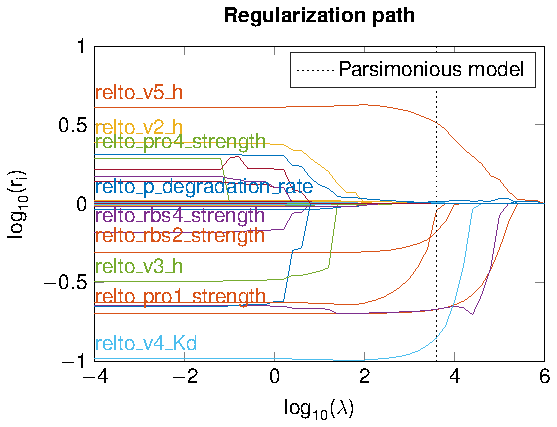
\includegraphics[width=110pt]{Figures/l1_tree.pdf}~~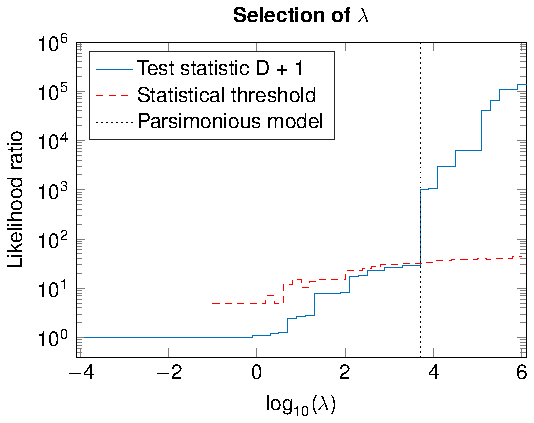
\includegraphics[width=110pt]{Figures/l1_selection.pdf}}
%\centerline{\includegraphics{fig01.eps}}
\caption{Left: Regularization path of a representative setup. On the x-axis, the regularization weight $\lambda$ is depicted. As $\lambda$ is increased, the number fold-changes unequal to zero is reduced and the estimates are shrinked towards zero. The labels are not exhaustive. As expected for non-linear models, the individual paths are not necessarily monotonous. The vertical dashed lines depicts the \emph{parsimonious} model. Right: Selection of $\lambda$. The likelihood-ratio test statistic $D$ is calculated for each value of $\lambda$ (blue solid line). The value where $D$ crosses the statistical threshold $\chi^2_{m_\lambda,0.05}$ (dashed red line) marks the \emph{parsimonious model} (dashed black line). To enable plotting in log-space, one is added to all quantities.}\label{fig:05}
\end{figure}

\begin{figure}[!tpb]%figure1
\centerline{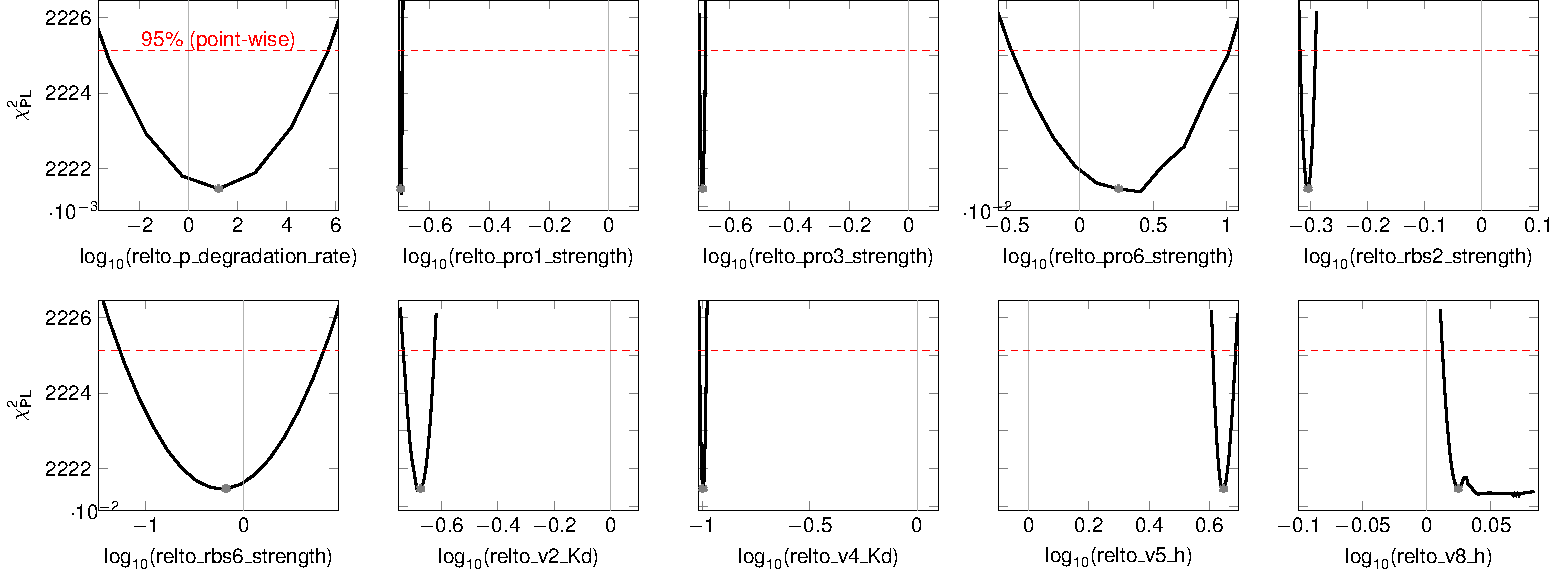
\includegraphics[width=235pt]{Figures/multi_plot.pdf}}
\caption{Determining fold-changes that are compatible with zero (gray vertical line) using \emph{PL}. Both parameters in the first column, and the one in the first row, fourth column are compatible with zero. These were actually false positives that could be transformed into true negatives by this analysis.}\label{fig:06}
\end{figure}

\begin{figure}[!tpb]%figure1
\centerline{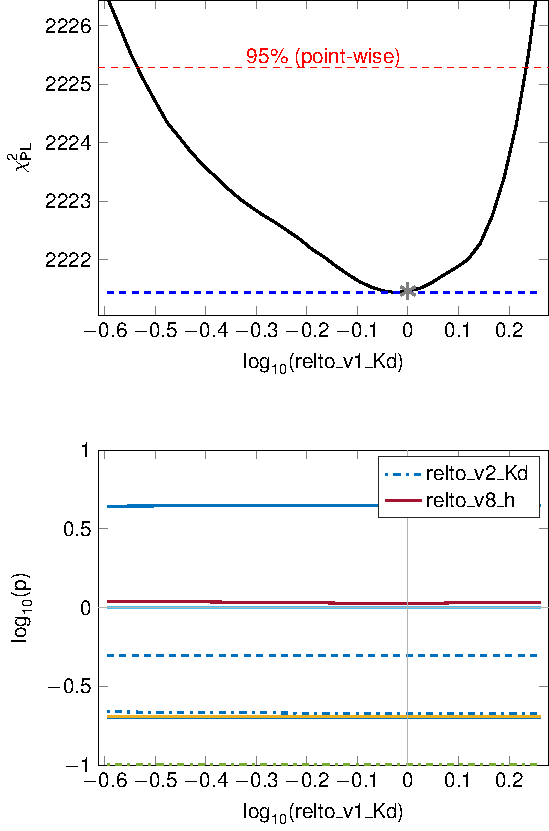
\includegraphics[width=110pt]{Figures/uniqueness_1.pdf}~~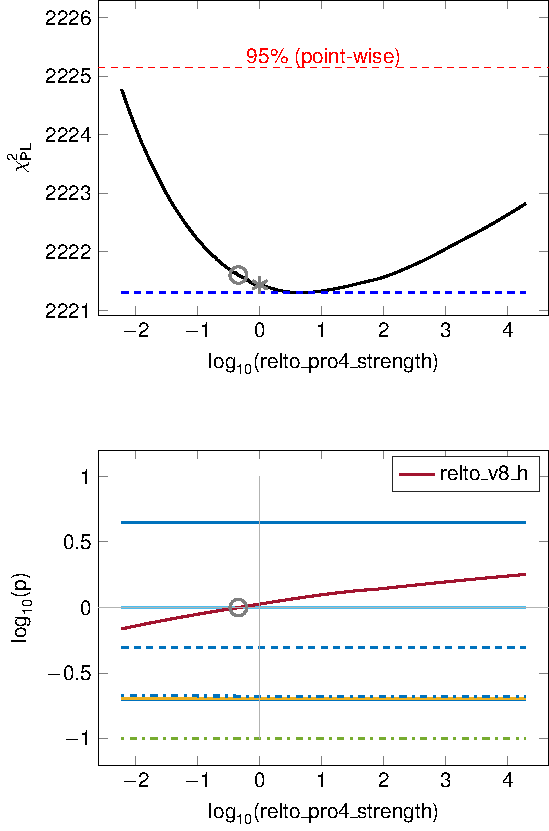
\includegraphics[width=110pt]{Figures/uniqueness.pdf}}
\caption{Uniqueness and exchangeability. To check the uniqueness of a solution we used the \emph{PL} whether ($r_i=0$ and $r_j\neq0$) gives an equivalent results as ($r_i\neq0$ and $r_j=0$) for $i\neq j$. The results of the supervised examination example are shown. In the upper row, \emph{PL} of a fold-change parameter that was estimated to zero is shown. The optimum (asterisk) is not at the minimum because the unbiased solution is computed. On the lower row, the respective values of the other $\{r_i\}$ are shown. When a parameter that was non-zero is compatible with zero, it is marked with a circle. On the left hand side the fold-change parameter of $K_{D,1}$, which is a true negative, cannot be exchanged with any other parameter. However, on the right hand side, a false negative fold-change $r_{pro4}$ could be exchanged with the false positive Hill coefficient $r_{H8}$. Thus although the solution classifies both parameters incorrectly, it pinpoints the possibility of the correct solution. Given the available data, these cannot be distinguished and experimental design would be necessary to decide which one is cell type-specific, or both.}\label{fig:07}
\end{figure}


%Text Text Text Text Text Text  Text Text Text Text Text Text Text
%Text Text  Text Text Text Text Text Text.
%Figure~2\vphantom{\ref{fig:02}} shows that the above method  Text
%Text Text Text  Text Text Text Text Text Text  Text Text.
%\citealp{Boffelli03} might want to know about  text text text text
%
%
%Table~\ref{Tab:01} shows that Text Text Text Text Text  Text Text
%Text Text Text Text. Figure~2\vphantom{\ref{fig:02}} shows that
%the above method Text Text. Text Text Text  Text Text Text Text
%Text Text. Figure~2\vphantom{\ref{fig:02}} shows that the above
%method Text Text. Text Text Text  Text Text Text Text Text Text.
%Figure~2\vphantom{\ref{fig:02}} shows that the above method Text
%Text.









%%%%%%%%%%%%%%%%%%%%%%%%%%%%%%%%%%%%%%%%%%%%%%%%%%%%%%%%%%%%%%%%%%%%%%%%%%%%%%%%%%%%%
%
%     please remove the " % " symbol from \centerline{\includegraphics{fig01.eps}}
%     as it may ignore the figures.
%
%%%%%%%%%%%%%%%%%%%%%%%%%%%%%%%%%%%%%%%%%%%%%%%%%%%%%%%%%%%%%%%%%%%%%%%%%%%%%%%%%%%%%%






\section{Discussion}
% Differences to linear setting
In this manuscript, we used $L_1$ regularization to predict cell type-specific parameters in systems of coupled partially observed ODEs.
Compared to the classical \emph{LASSO} which was designed for linear models, many pitfalls emerge for parameter estimation in non-linear ODE systems.
Therefore, we augmented an available implementation by $L_1$ peculiarities
and thereby focused on optimization routines that can efficiently handle non-linearity.
Although, we cannot exclude that the presented methodolgy may be improved in terms of numerical performance by concepts presented in the vast amount of literature on extending \emph{LASSO}, 
we could implement a robust and numerically stable algorithm.
In our example, cell type-specific parameters were reliably predicted for 500 different data setups.

Because model predictions non-linearly depend on parameters, 
the regularization paths depicting the dependency of the cell specific parameters on the regularization strength 
are not necessarily monotonous and even the sign of the individual $L_1$ penalty terms may change.
Therefore the regularization paths have to be calculated by discretely scanning $\lambda$ 
instead of calculating the paths for whole intervals as it is feasible for linear systems.

% Uniqueness and local optima
Local optima are of major concern in partially observed non-linear ODE systems.
An established method to discover local optima is to perform multi-start deterministic optimization and compare the results.
For different $\lambda$, other local optima could become globally optimal or even new, additional optima could emerge for a specific range of $\lambda$.
To circumvent such issues, the multi-start optimization could be applied for each value of $\lambda$.
However, comprehensively sampling the parameter space by such a strategy is usually computationally infeasible for most realistic models.
Therefore, the approach we applied is finding the global optimum for each cell type individually and then gradually increase $\lambda$ using the latest fit as initial guess.

{\bf Identified differences between cell types may not be unique, i.e. a difference could be exchanged with a parameter that is cell type-independent without significantly changing the fit.
Due to identifiability issues, $L_1$ regularized parameters can compensate each other resulting a piecewise flat \emph{PL}.
Although only detectable by heuristics or supervised examination, only a subgroup of such coupled parameters are necessary to be different.}

% Numerics
Most optimization algorithms efficiently handle least squares problems but have shortcomings for $L_1$ regularized optimization.
A key challenge that we faced was that numerics became problematic for parameters in the vicinity of zero.
For Gauss-Newton steps, the curvature / Hessian
\begin{equation}
	H_{ij} \approx \text{sres}_{ii} \cdot \text{sres}_{jj} = \frac{\text{sgn}(r_i)}{\frac{2}{\lambda}\sqrt{\frac{|r_i|}{1/\lambda}}} \cdot \frac{\text{sgn}(r_j)}{\frac{2}{\lambda}\sqrt{\frac{|r_j|}{1/\lambda}}} \:.
\end{equation}
is approximated by the first-order derivatives $\text{sres}_{i}$.
In this case, $r_i$ appears in the denominator. Therefore, as $r_i$ approaches zero, the Hessian
\begin{equation}
	\lim_{r_i \rightarrow 0} H_{ij} = \lim_{r_j \rightarrow 0} H_{ij} = \pm \infty
\end{equation}
diverges.
For large entries in the Hessian, the optimizer decreases the step size and therefore may get stuck when approaching zero.
Thereby, the FPR is increased since parameters compatible with zero shrink but may not be able to actually reach zero.
We conclude that the FPR could be further improved if such numerical issues are completely solved. %numerics are the major source of FPR in our implementation.
To overcome these limitations, norms with $k>1$ could be employed.
Although in the proximity of zero $L_1$ dominates the Hessian, an additional $L_2$ term like in the \emph{elastic net} could provide enough directional information to come closer to zero.
We postpone this analysis to future research.

% Manual inspection

% Cross-validation
%Another strategy frequently used to choose $\lambda$ is cross-validation.
%However, further analysis would be necessary for defining a good sampling strategy.
Another remaining open question is to which extent cross-validation strategies are applicable in the Systems Biology setting.
A basic assumption for cross-validation is that the drawn subsets contain qualitatively the same information than the original, full data set.
This assumption, however, is violated for pathway models and manifests in a strong dependency of parameter identifiability on resampled data and the experimental setup.
The latter originates from the complex grouping structure of measurements given by common treatment conditions, jointly observed dynamic states, as well as by available sampling times.


% Other directions
% Shrinkage
% L2 with analysis of shape

%DREAM specific discussion
We chose a benchmark model from the \emph{DREAM6} parameter estimation challenge 
to demonstrate applicability of our implementation because it provides a variety of predefined realistic experimental setups.
For assessing the performance, cell type dependencies of parameters were introduced and then recovered in an unsupervised manner.
Compared to typical pathway models, the \emph{DREAM6} setting exhibits two major simplifications.
First, the components of the reaction network are directly observed, i.e.~there are no scaling parameters.
Second, the initial concentrations were assumed as known.
However, we do not expect issues if both simplifications are relaxed because the unregularized parameter estimation implementation is well-tested for such cases.

In partially observed non-linear ODE systems, it has been shown that non-identifiability is of major concern.
A non-identifiable parameter can be associated with a flat \emph{PL}, i.e. the effect on observed quantities by changing one parameter can be compensated by others.
If the range of a fold-change parameter is compatible with zero, the $L_1$ regularization will force the estimate to zero.
Hence, the presence of non-identifiabilites may decrease the TPR.
One example for such a behavior are Hill kinetics, i.e. Hill coefficients and $K_D$ values, which also appeared as most difficult to detect.
We conclude that identifiability is limiting the TPR in this setting.
%Experimental design principles were not applied, which were the task in the original DREAM6 challenge.
%Therefore, one cannot expect perfect detection of cell type-specific parameters due to identifiability issues.
Since the subset of available data sets was randomly drawn from the predefined set of experiments,
it is not expected that all subsets contain comprehensive information for estimating all parameters.
Therefore, identifiability issues naturally occur and appear as false negatives in the parameter selection step.
In general, the magnitude of both, correct and incorrect predictions depend on the amount and quality of data, as well as on the size of the underlying differences.

It has to be stated that cell type differences are detected only if there is evidence in the data.
Therefore, unobserved components and specific, incomplete measurement conditions increase the chance of missing biologically relevant cell-specific characteristics.
However, we could show that the unbiased estimates of true positive fold-changes are robust to missclassification of others.
Nevertheless, the final model should always be checked for biological completeness and plausiblity.

In summary, we proposed to use $L_1$ regularization in combination with nonlinear models based on \emph{ordinary differential equation} systems.
Theoretical considerations were given and the approach was tested for random designs of a \emph{DREAM} benchmark model.
The ability to improve the results using the \emph{profile likelihood} was demonstrated.
Concludingly, the presented methodology is shown to facilitate detection relevant differences between dynamical models of cell types, which is an important step towards discovering drug targets specifically affecting cells of interest.

\section*{Acknowledgements}

We thank Marcel Schilling, Ruth Merkle, and Ursula Klingm{\"u}ller for biological motivation of the topic.
Further, we thank Daniel Kaschek and Helge Hass for discussion on the theoretical side.

\section*{Funding}

This work was supported by the German Ministry of Education and Research through the grants LungSys II (Grant No. 0316042G), SBEpo (Grant No. 0316182B), and IMOMESIC (Grant No. 031A604B)]. 

\bibliographystyle{natbib}
%\bibliographystyle{achemnat}
%\bibliographystyle{plainnat}
%\bibliographystyle{abbrv}
% \bibliographystyle{bioinformatics}

% \bibliographystyle{plain}

\bibliography{document}

\end{document}
